\documentclass{beamer}

\usepackage{ucs}
\usepackage[utf8x]{inputenc}
\usepackage[T1]{fontenc}
\usepackage[english]{babel}

\usepackage{graphicx}
\usepackage{multirow}%	multirow
\usepackage[retainorgcmds]{IEEEtrantools}%	IEEEeqnarray
\usepackage{hyperref}%	hyperreferences
\usepackage[noabbrev]{cleveref}%	clever reference text
\usepackage{relsize}%	relative font sizes
\usepackage{listings}

%	presentation info
\title{JSARToolKit}
\subtitle{Augmented Reality applied to a Pokémon\textsuperscript{\textregistered}\ Game}

\author[A.C.Macedo \and M.Palhas \and P.Costa]{Ana Catarina Macedo
\and Miguel Palhas
\and Pedro Costa}

\institute[]{
	University of Minho\\
	Department of Informatics
}

\date{Braga, June 2012}


%	beamer options
\usetheme{CambridgeUS}


\begin{document}%	begin presentation

\frame[plain]{\titlepage}

\frame{\frametitle{Index}\tableofcontents}




\section{The Project}
\begin{frame}
	\frametitle{Concept}
	\begin{itemize}
		\item{A Pokémon\textsuperscript{\textregistered} game
		\begin{itemize}
			\item{Based on the original Nintendo\textsuperscript{\textregistered} Game Boy\textsuperscript{\textregistered} game;}
		\end{itemize}
		}
		\item{Interaction using Augmented Reality;
		\begin{itemize}
			\item{Using JSARToolKit;}
		\end{itemize}
		}
	\end{itemize}
	
	\begin{figure}
		\begin{center}
			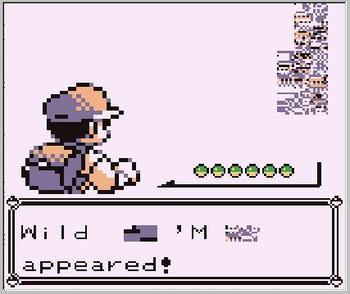
\includegraphics[width=0.4\textwidth]{slides/images/missingno.jpeg}
			\;
			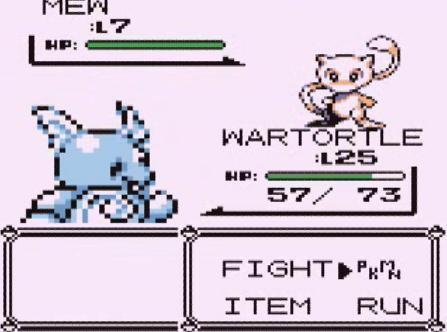
\includegraphics[width=0.4\textwidth]{slides/images/mew.png}
		\end{center}
	\end{figure}
\end{frame}

\begin{frame}
	\frametitle{Goals}
	\begin{enumerate}
		\item{Use the webcam through the browser;}
		\item{Use the JSARToolKit to recognize the patterns seen by the webcam;}
		\item{Use WebGL to add virtual elements;}
		\item{Identify the individual markers and the user interaction;}
		\item{Implement the game mechanics;}
	\end{enumerate}
	
	\begin{block}{Tools}
		\begin{itemize}
			\item{Google Chrome + WebRTC (experimental);}
			\item{Javascript + \textit{Three.js} (WebGL);}
			\item{JSARToolKit;}
		\end{itemize}
	\end{block}
\end{frame}





\section{The Game}
\begin{figure}
	\frametitle{The Game}
	\begin{columns}
		\begin{column}{0.5\linewidth}
			\tableofcontents[currentsection,subsectionstyle=show/show/hide]
		\end{column}
		\begin{column}{0.5\linewidth}
			\begin{figure}
				\begin{center}
					
\includegraphics[width=\linewidth]{slides/images/pikachu.jpeg}
				\end{center}
			\end{figure}
		\end{column}
	\end{columns}
\end{figure}

\subsection{Augmented Reality}
\begin{frame}
	\frametitle{Augmented Reality}
	\begin{itemize}
		\item{Similar to the \texttt{simpletest} sample:
		\begin{itemize}
			\item{Identifies markers in the scene;}
			\item{Retrieves the transformation matrices;}
			\item{Places virtual elements ``on'' the markers;}
		\end{itemize}
		}
	\end{itemize}
	
	\begin{figure}
		\begin{center}
			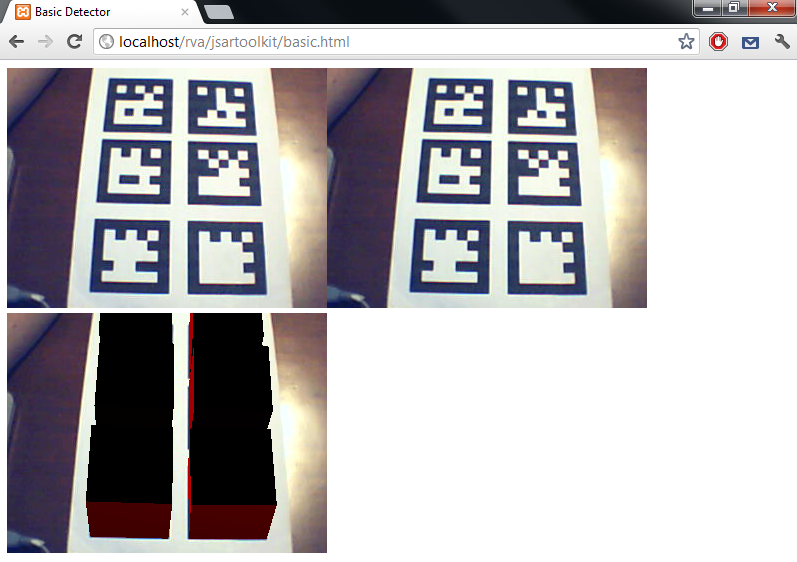
\includegraphics[width=0.6\linewidth]{slides/images/basic.png}
		\end{center}
	\end{figure}
\end{frame}

\subsection{Mechanics}
\begin{frame}
	\frametitle{}
	\begin{columns}
		\begin{column}{0.5\linewidth}
		\end{column}
		\begin{column}{0.5\linewidth}
		\end{column}
	\end{columns}
\end{frame}

\subsection{Features}

\section{Conclusion}
\subsection{Problems}




\section{Questions}
\begin{frame}
	\titlepage
	\begin{center}
		\Huge\bfseries
		- ? -
	\end{center}
\end{frame}

\end{document}%	end presentation